\subsection{Choice of BLAS Library}
\label{subseq:blas-comparison}


To perform columns elimination of fully summed block of frontal matrices, MUMPS intensively uses GEMM, TRSM and GETRF subroutines which are parts of BLAS and LAPACK libraries. As an example, figure \ref{fig:mumps:steps-of-type-2-factorization} demonstrates factorization of a type 2 node.\\


\figpointer{\ref{fig:mumps:type-2-frontal-matrix}}
\begin{figure}[htpb]
  \centering
  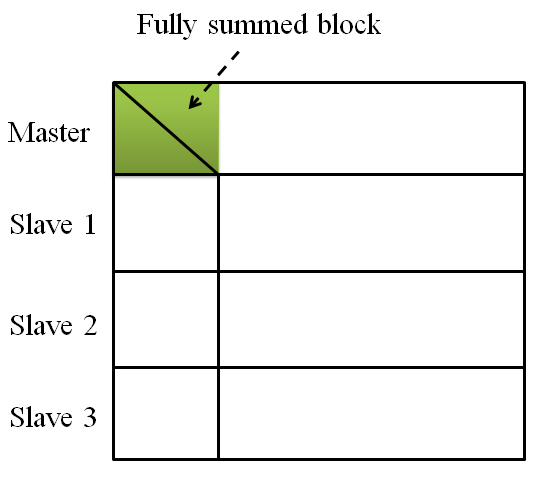
\includegraphics[width=0.45\textwidth]{figures/chapter-2/mumps-type-2-frontal-matrix.png}
\caption{MUMPS: static and dynamic scheduling}
\label{fig:mumps:type-2-frontal-matrix}
\end{figure}


\figpointer{fig:mumps:steps-of-type-2-factorization}
\begin{figure}[htpb]
  \centering
  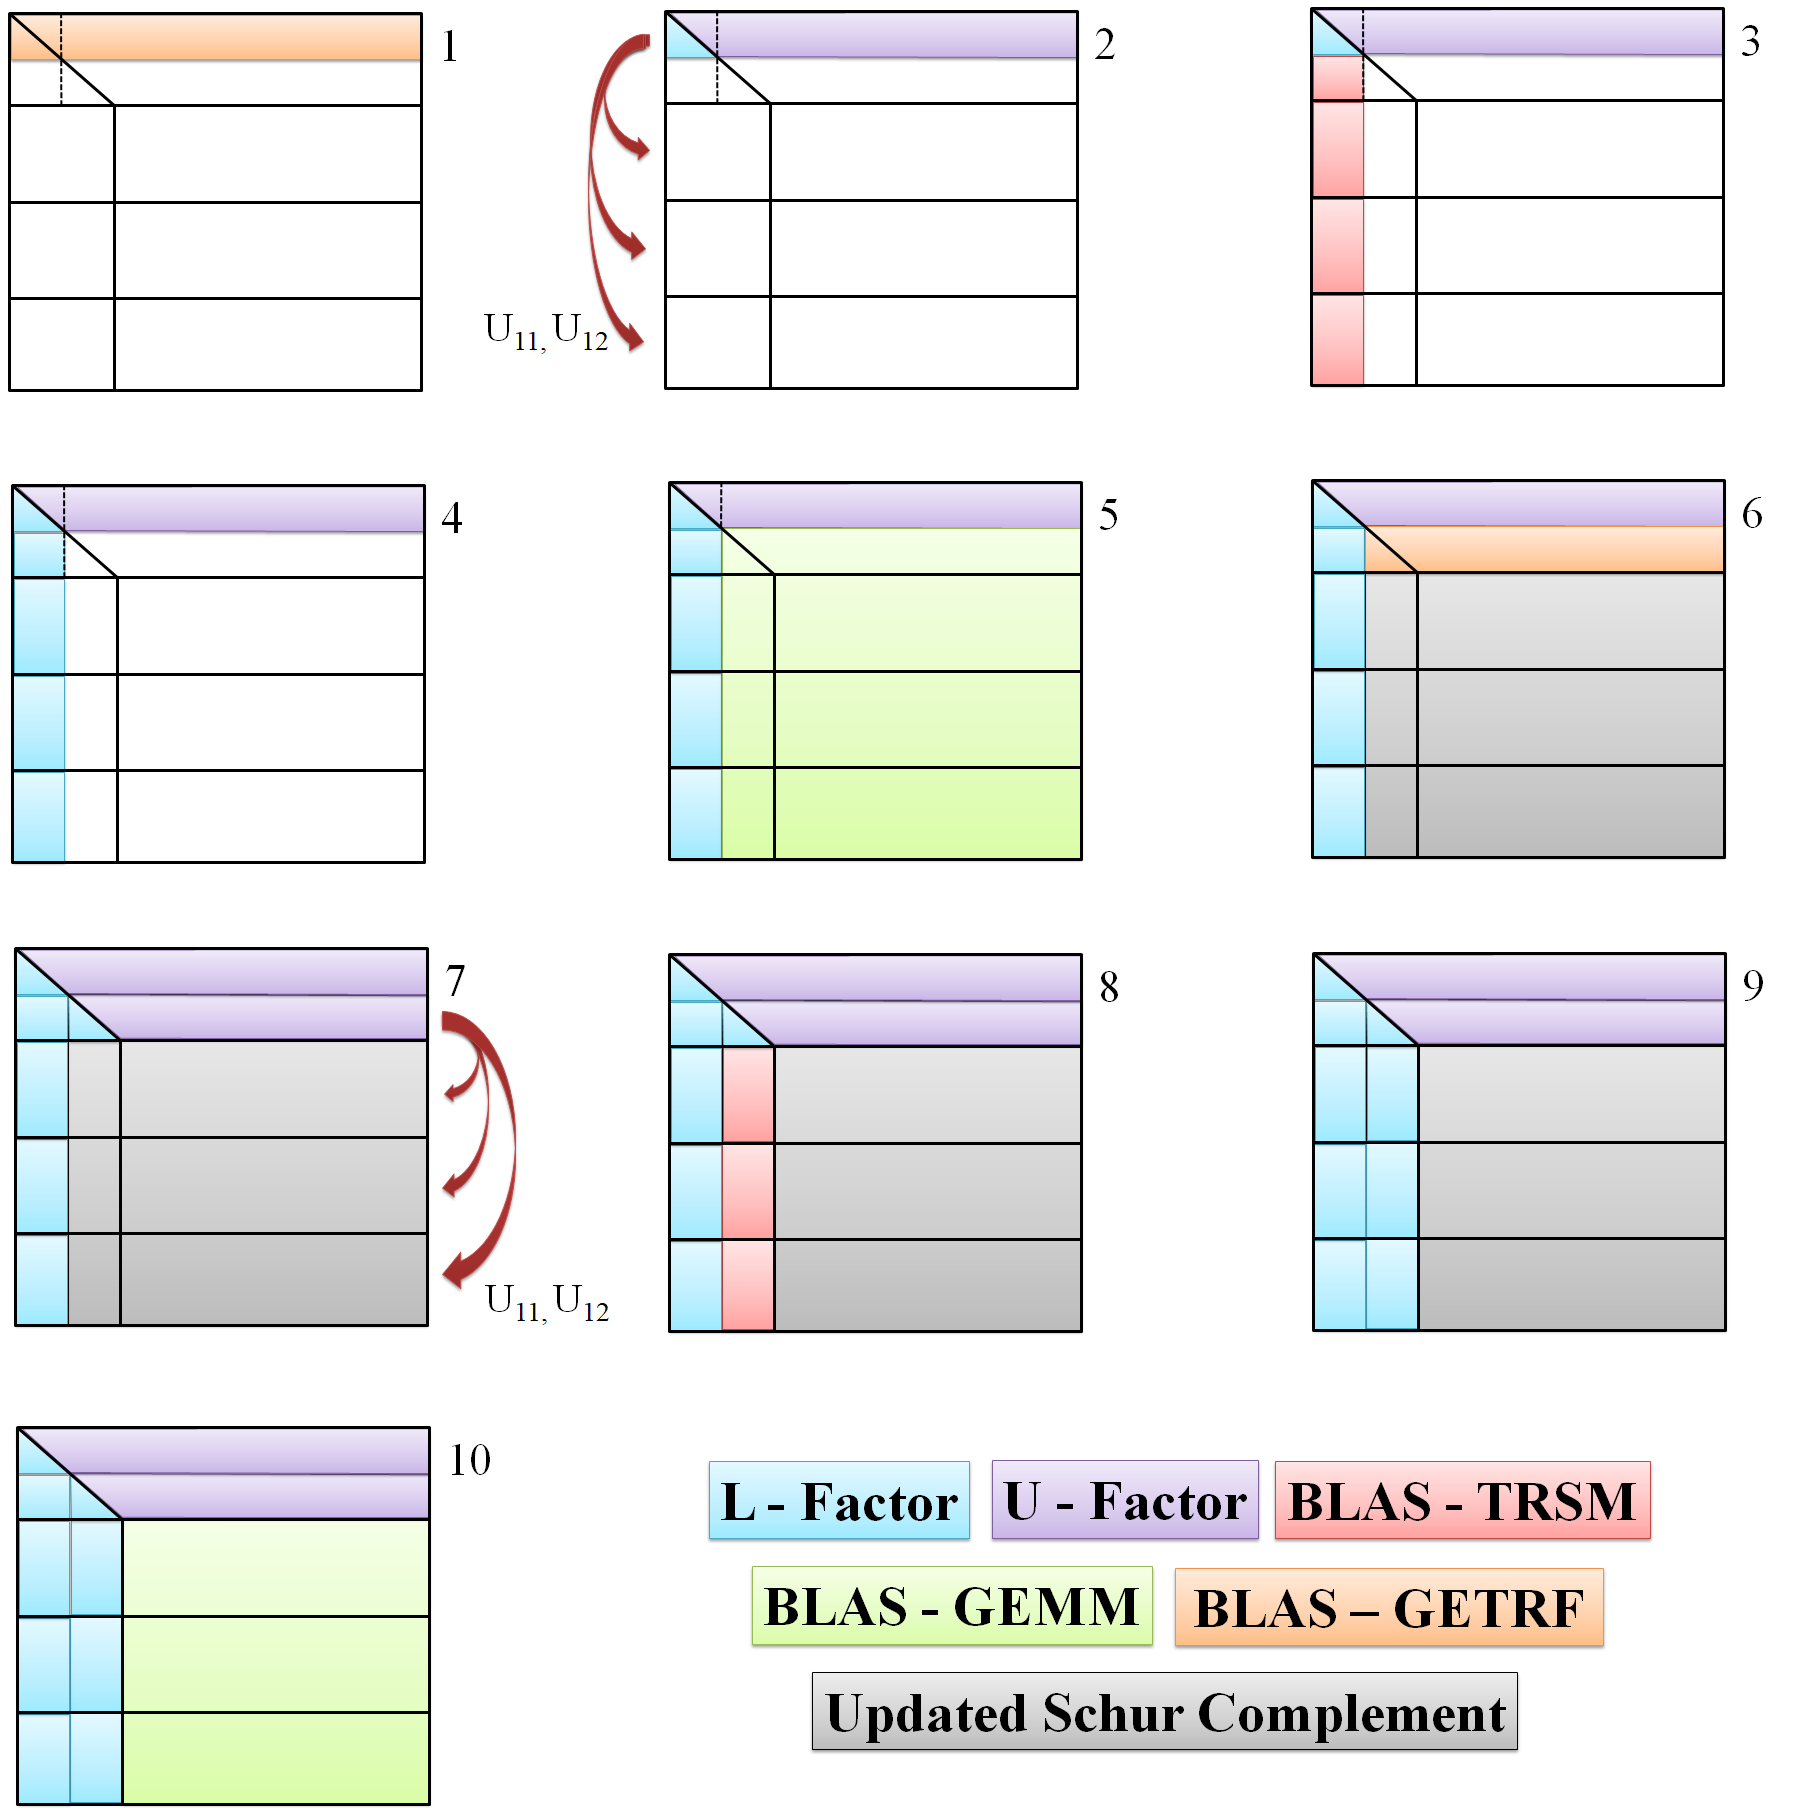
\includegraphics[width=0.85\textwidth]{figures/chapter-2/mumps-type-2-part-1.png}
\caption{MUMPS: An example of a type 2 node factorization}
\label{fig:mumps:steps-of-type-2-factorization}
\end{figure}


Both BLAS and LAPACK originate from the Netlib project which is a repository of numerous scientific computing software maintained by AT\&T Bell Laboratories, the University of Tennessee, Oak Ridge National Laboratory and other scintific communities \cite{netlib-overview}.\\


The goal of BLAS library is provision of a high efficient implementation of common dense linear algebra kernels by means of high rate of floating point operations per memory access, low cache and Translation Lookaside Buffer (TLB) miss rates.\\


In its turn, LAPACK is designed in such a way so that as much as possible computations is performed by calls to BLAS library. This allows to achieve high efficiency for operations such as $LU$, $QR$, $SVD$ decompositions, triangular solve, etc. on modern computers. However, the Netlib BLAS implementation is written for an abstract general-purpose central processing unit, in mind, where hardware parameters are based on market statistics. Hence, it is not possible to achieve the maximum possible performance on a specific machine.\\


Hence, there exist special-purpose, hardware-specific implementations of the library developed by hardware vendors i.e. IBM, Cray, Intel, AMD, etc., as well as open-source tuned implementations such as ATLAS, OpenBLAS, etc. To achieve full compatibility, the developers consider the Netlib implementation of BLAS library as the standard (or reference) and thus overwrite all subroutines with additional tuning and optimization. This approach makes it possible to easily replace different BLAS implementations during object files linking  without any modifications of the source code.\\
 

Table \ref{table:list-of-blas-implementations} shows commercial and open-source tunned BLAS implementations available on the market today.\\

\begin{table}[h!]
\centering
\small
\begin{tabular}{|c|c|c|}
\hline
Name                                                                 & Description                                                                                                                                                 & License                                                       \\ \hline
Accelerate                                                           & Apple's implementation for macOS and iOS                                                                                                                    & \begin{tabular}[c]{@{}c@{}}proprietary\\ license\end{tabular} \\ \hline
ACML                                                                 & BLAS implementation for AMD processors                                                                                                                      & \begin{tabular}[c]{@{}c@{}}proprietary\\ license\end{tabular} \\ \hline
C++ AMP                                                              & Microsoft's AMP language extension for Visual C++                                                                                                           & \begin{tabular}[c]{@{}c@{}}open\\ source\end{tabular}         \\ \hline
ATLAS                                                                & Automatically tuned BLAS implementation                                                                                                                     & \begin{tabular}[c]{@{}c@{}}open\\ source\end{tabular}         \\ \hline
Eigen BLAS                                                           & \begin{tabular}[c]{@{}c@{}}BLAS implemented on top of \\ the MPL-licensed Eigen library\end{tabular}                                                        & open source                                                   \\ \hline
ESSL                                                                 & optimized BLAS implementation for  IBM's machines                                                                                                           & \begin{tabular}[c]{@{}c@{}}proprietary\\ license\end{tabular} \\ \hline
GotoBLAS                                                             & Kazushige Goto's implementation of BLAS                                                                                                                     & \begin{tabular}[c]{@{}c@{}}proprietary\\ license\end{tabular} \\ \hline
HP MLIB                                                              & \begin{tabular}[c]{@{}c@{}}BLAS implementation supporting IA-64, PA-RISC, x86 \\ and Opteron architecture\end{tabular}                                      & \begin{tabular}[c]{@{}c@{}}proprietary\\ license\end{tabular} \\ \hline
Intel MKL                                                            & \begin{tabular}[c]{@{}c@{}}Intel's implementation of BLAS optimized for\\ Intel Pentium, Core,  Xeon and Xeon Phi\end{tabular}                              & \begin{tabular}[c]{@{}c@{}}proprietary\\ license\end{tabular} \\ \hline
Netlib BLAS                                                          & The official reference implementation on Netlib                                                                                                             & \begin{tabular}[c]{@{}c@{}}open\\ source\end{tabular}         \\ \hline
OpenBLAS                                                             & Optimized BLAS library based on GotoBLAS                                                                                                                    & \begin{tabular}[c]{@{}c@{}}open\\ source\end{tabular}         \\ \hline
PDLIB/SX                                                             & BLAS library targeted to the NEC SX-4 system                                                                                                                & \begin{tabular}[c]{@{}c@{}}proprietary\\ license\end{tabular} \\ \hline
SCSL                                                                 & BLAS implementations for SGI's Irix workstations                                                                                                            & \begin{tabular}[c]{@{}c@{}}proprietary\\ license\end{tabular} \\ \hline
\begin{tabular}[c]{@{}c@{}}Sun\\ Performance \\ Library\end{tabular} & \begin{tabular}[c]{@{}c@{}}Optimized BLAS and LAPACK for SPARC, Core \\ and AMD64 architectures under \\ Solaris 8, 9, and 10 as well as Linux\end{tabular} & \begin{tabular}[c]{@{}c@{}}proprietary\\ license\end{tabular} \\ \hline
\end{tabular}
\caption{Commercial and open source BLAS implementations \cite{wiki:blas-implementations}}
\label{table:list-of-blas-implementations}
\end{table}



Among all libraries listed in table \ref{table:list-of-blas-implementations} there were only four available on HW1 machine, namely: Netlib BLAS, Intel MKL, OpenBLAS and ATLAS. However, installation of ATLAS requires to switch off dynamic frequency scaling, also called CPU throttling, to allow an ATLAS configuration routines to find the best loop transformation parameters for a specific hardware. In order to turn off CPU throttling, one has to reboot the entire machine and make appropriate changes in Basic Input/Output System (BIOS). This fact made ATLAS library not suitable for the rest of the study and we excluded it from the primary list of candidates. Moreover, during installation, one has to explicitly provide the number of OpenMP threads that are going to be used once a BLAS subroutine is called. This means there is no way to change the number of threads per MPI process in run-time without re-installation of ATALS library. Thus, only 3 versions of MUMPS-PETSc (Netlib BLAS, Intel MKL and OpenBLAS) library were compiled, installed and tested with using both GRS and SuiteSparse matrix sets and 1 thread per MPI process. The test results are obtained on HW1 machine only are represented in figures \ref{fig:mumps-blas-configuration-1}, \ref{fig:mumps-blas-configuration-2} and appendix \ref{app:app-blas-configuration}.\\


\figpointer{\ref{fig:mumps-blas-configuration-1}}
\begin{figure}[htpb]
\centering
	\begin{tabular}{cc}
		\subfloat[k3-18]{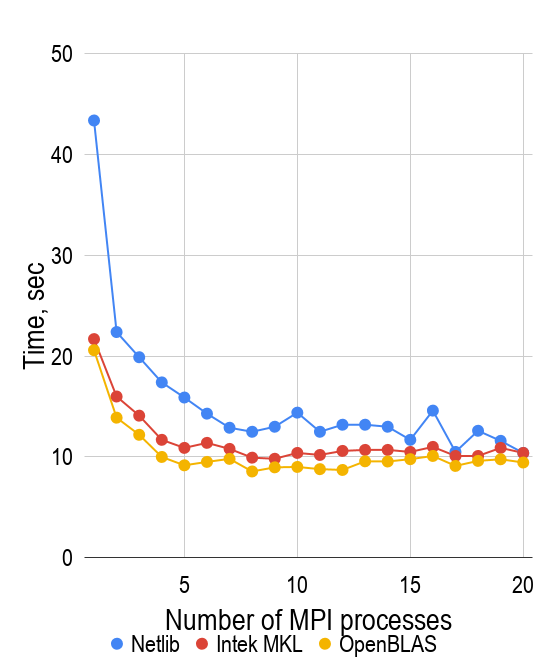
\includegraphics[width=0.48\textwidth]{figures/chapter-2/blas-configuration/k3-18.png}} &
		\subfloat[cube-645]{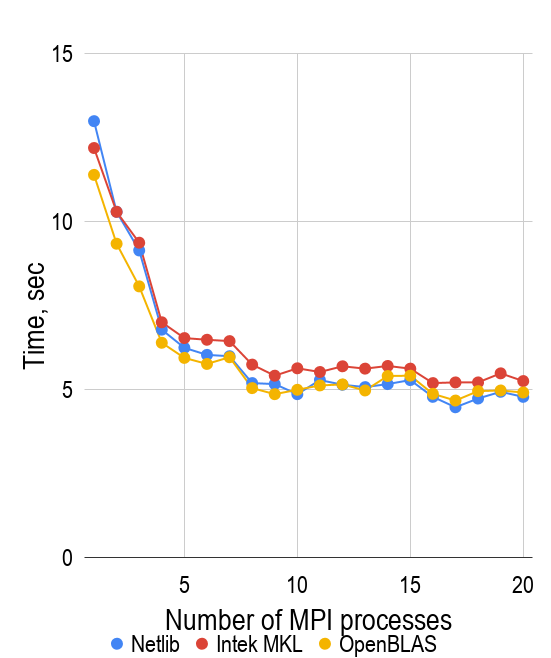
\includegraphics[width=0.48\textwidth]{figures/chapter-2/blas-configuration/cube-645.png}} \\
		\subfloat[k3-2]{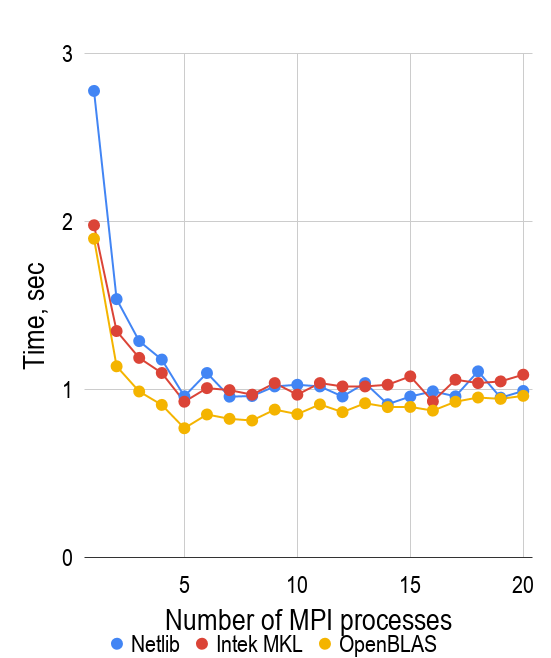
\includegraphics[width=0.48\textwidth]{figures/chapter-2/blas-configuration/k3-2.png}} &
		\subfloat[cube-64]{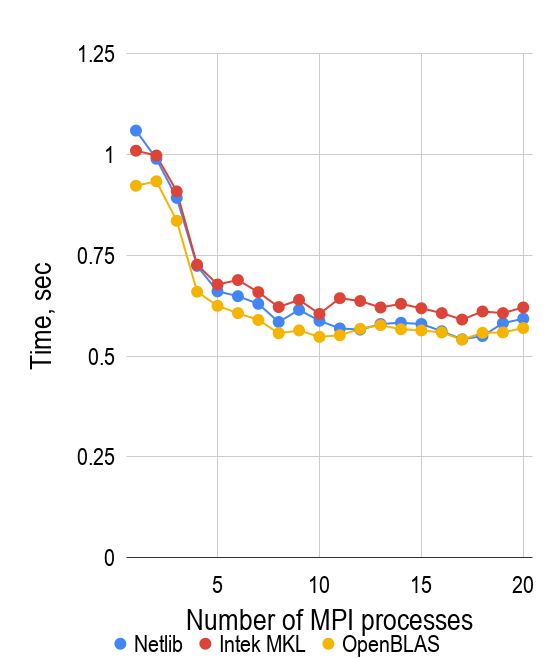
\includegraphics[width=0.48\textwidth]{figures/chapter-2/blas-configuration/cube-64.png}} \\
	\end{tabular}
	\caption{MUMPS: comparison of different BLAS libraries with using GRS matrix set on HW1 machine}
	\label{fig:mumps-blas-configuration-1}
\end{figure}


\figpointer{\ref{fig:mumps-blas-configuration-2}}
\begin{figure}[htpb]
\centering
	\begin{tabular}{cc}
		\subfloat[cube-5]{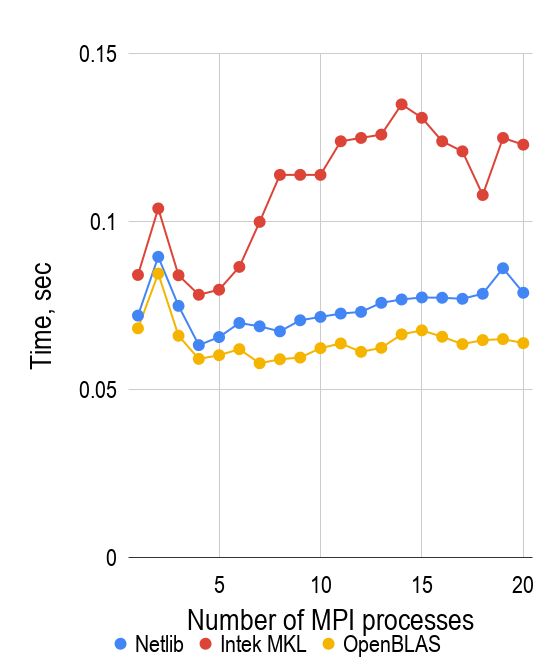
\includegraphics[width=0.43\textwidth]{figures/chapter-2/blas-configuration/cube-5.png}} &
		\subfloat[pwr-3d]{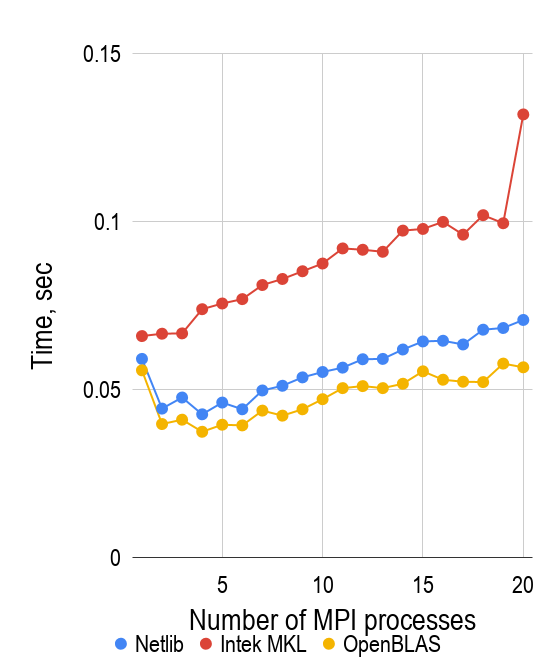
\includegraphics[width=0.43\textwidth]{figures/chapter-2/blas-configuration/pwr-3d.png}} \\
		\subfloat[memchip]{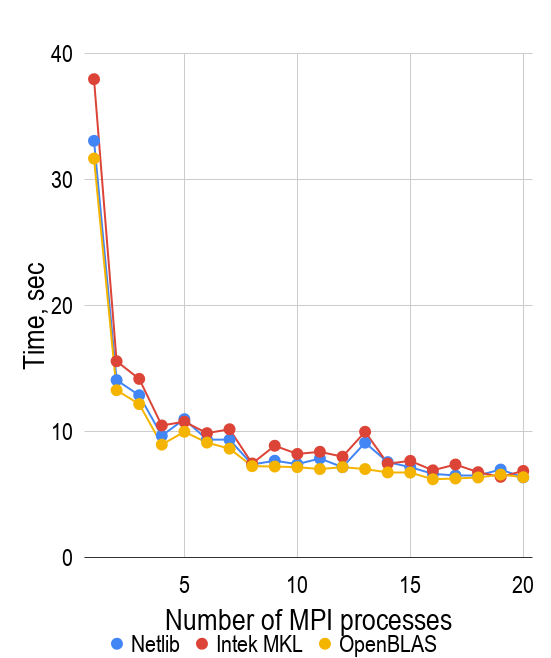
\includegraphics[width=0.48\textwidth]{figures/chapter-2/blas-configuration/memchip.png}} & \subfloat[torso3]{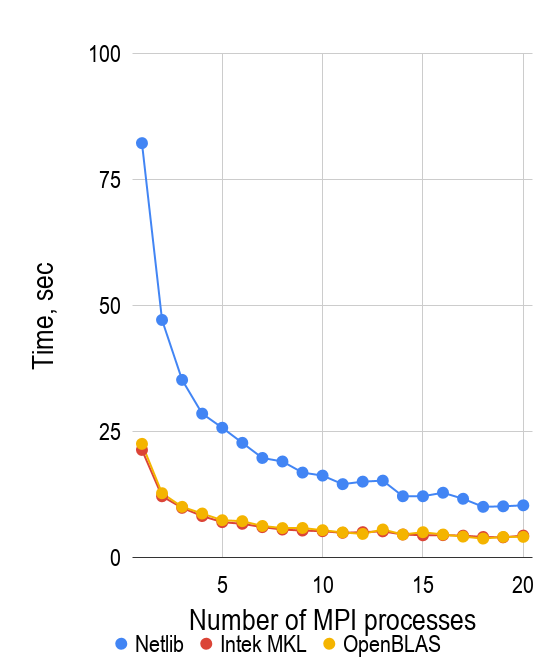
\includegraphics[width=0.48\textwidth]{figures/chapter-2/blas-configuration/torso3.png}} \\
	\end{tabular}
	\caption{MUMPS: comparison of different BLAS libraries with using both GRS and SuiteSparse matrix sets on HW1 machine}
	\label{fig:mumps-blas-configuration-2}
\end{figure}



The tests show that OpenBLAS outperforms both Netlib and Intel MKL libraries in case of GRS matrix set. In average, OpenBLAS is about \textbf{13\%} faster than the default Netlib implementation and approximately \textbf{21\%} faster than Intel MKL library. It is interesting to notice Intel MKL turned out to be slower than the default Netlib BLAS implementation for small and medium size GRS matrices in almost \textbf{52\%} and \textbf{2\%}, respectively.At the same time, both tuned libraries, OpenBLAS and Intel MKL, showed significant performance gain relatively to the standard Netlib BLAS implementation in case of SuiteSparse matrix set. The libraries reduced the execution time in almost \textbf{50\%} in average. In opposite to GRS matrix set, it turned out that Intel MKL was often faster than OpenBLAS for almost all test cases from SuiteSparse matrix set. However, the difference between them is negligibly small. The result of comparison are summarized in tables \ref{table:mumps-blas-performance-gain-grs} and \ref{table:mumps-blas-performance-gain-suitesprase}.\\


\begin{table}[h!]
\centering
\begin{tabular}{|c|c|c|c|}
\hline
\begin{tabular}[c]{@{}c@{}}Matrix\\ Name\end{tabular} & \begin{tabular}[c]{@{}c@{}}Performance\\ gain of \\ OpenBLAS \\ relatively to \\ Netlib \%\end{tabular} & \begin{tabular}[c]{@{}c@{}}Performance\\ gain of\\ IntelMKL\\ relatively to\\ Netlib \%\end{tabular} & \begin{tabular}[c]{@{}c@{}}Performance\\ gain of\\ OpenBLAS\\ relatively to\\ Intel MKL \%\end{tabular} \\ \hline
pwr-3d                                                & 14.607                                                                                                  & -56.249                                                                                              & 44.695                                                                                                  \\ \hline
cube-5                                                & 13.569                                                                                                  & -47.797                                                                                              & 39.931                                                                                                  \\ \hline
cube-64                                               & 4.385                                                                                                   & -5.483                                                                                               & 9.323                                                                                                   \\ \hline
cube-645                                              & 1.897                                                                                                   & -7.474                                                                                               & 8.702                                                                                                   \\ \hline
k3-2                                                  & 13.906                                                                                                  & 0.833                                                                                                & 13.057                                                                                                  \\ \hline
k3-18                                                 & 29.914                                                                                                  & 21.03                                                                                                & 11.29                                                                                                   \\ \hline
\end{tabular}
\caption{Comparison of different MUMPS-BLAS configurations applied to GRS matrix set}
\label{table:mumps-blas-performance-gain-grs}
\end{table}



\begin{table}[h!]
\centering
\begin{tabular}{|c|c|c|c|}
\hline
\begin{tabular}[c]{@{}c@{}}Matrix\\ Name\end{tabular} & \begin{tabular}[c]{@{}c@{}}Performance\\ gain of \\ OpenBLAS \\ relatively to \\ Netlib \%\end{tabular} & \begin{tabular}[c]{@{}c@{}}Performance\\ gain of\\ IntelMKL\\ relatively to\\ Netlib \%\end{tabular} & \begin{tabular}[c]{@{}c@{}}Performance\\ gain of\\ OpenBLAS\\ relatively to\\ Intel MKL \%\end{tabular} \\ \hline
cant                                                  & 26.981                                                                                                  & 25.964                                                                                               & 1.233                                                                                                   \\ \hline
consph                                                & 67.617                                                                                                  & 68.252                                                                                               & -2.327                                                                                                  \\ \hline
CurlCurl\_3                                           & 78.804                                                                                                  & 79.37                                                                                                & -3.371                                                                                                  \\ \hline
Geo\_1438                                             & 83.106                                                                                                  & 83.565                                                                                               & -2.857                                                                                                  \\ \hline
memchip                                               & 6.066                                                                                                   & -6.909                                                                                               & 11.883                                                                                                  \\ \hline
PFlow\_742                                            & 75.574                                                                                                  & 74.943                                                                                               & 1.416                                                                                                   \\ \hline
pkustk10                                              & 35.089                                                                                                  & 34.536                                                                                               & 0.502                                                                                                   \\ \hline
torso3                                                & 66.185                                                                                                  & 66.988                                                                                               & -2.837                                                                                                  \\ \hline
x104                                                  & 41.82                                                                                                   & 41.936                                                                                               & -0.445                                                                                                  \\ \hline
\end{tabular}
\caption{Comparison of different MUMPS-BLAS configurations applied to SuiteSparse matrix set}
\label{table:mumps-blas-performance-gain-suitesprase}
\end{table}



In this section, we have shown how and where MUMPS utilizes common third-party libraries. The design of MUMPS can be considered as a good example of a scientific software architecture which reuses well-known, common blocks which appear quite often in scientific programs i.e. dense linear algebra kernels. Such design allows to easily configure and adopt software for a specific hardware which we demonstrated in this section.\\


We have also shown that MUMPS-OpenBLAS configuration is the best choice for GRS matrix set. It has been interesting to observe that the tuned Intel implementation of BLAS compiled with the latest Intel compiler demonstrated slow-down in contrast to the standard not optimized implementation. However, we can assume that amount of GRS test cases is not enough to make such a conclusion and thus the matrix set has to be extended considerably.\\